\documentclass[a4paper,12pt]{article}
\usepackage[dvipsnames, svgnames, x11names]{xcolor}
\usepackage{tikz}
\usepackage{arydshln} %tabular \hdashline
\usepackage[colorlinks,urlcolor=blue]{hyperref}

\usepackage[utf8]{inputenc}
% \usepackage[cp1251]{inputenc}
% \usepackage[russian]{babel}
% \usepackage{amssymb,amsmath}

\usepackage{layout} %layout


% \documentclass[a4paper]
% \paperwidth = 597pt
% \paperheight = 845pt
% 1 дюйм = 2.54cm

\oddsidemargin=0.46cm % arg отступ от левого края листа до текста, минус 1 дюйм.
\topmargin=-1.79cm % расстояние от верхнего края до верхнего колонтитула, минус 1 дюйм.

\textwidth=16.560831cm % arg ширина текста, для А4 типично arg = 16 cm.
\textheight=27.059719cm % arg высота текста, для А4 типично arg = 24 cm.

\pagestyle{empty} % стиль страниц, где arg может принимать значения:
% arg = empty % без колонтитулов и номеров страниц;
% arg = plain % без колонтитулов, номера страниц внизу в центре;
% arg = headings % колонтитулы генерируются автоматически;
% arg = myheadings % колонтитулы задаются пользователем.

\parindent=24pt % абзацный отступ
\parskip=0pt % интервал между абзацами
\tolerance=2000 % терпимость к "жидким" строкам
\flushbottom % выравнивание высоты страниц 

\marginparsep = 0pt
\marginparwidth = 0pt

\definecolor{Mtrs}{RGB}{2,57,68}
\definecolor{Mtrs1}{RGB}{78,97,40}

\usetikzlibrary{shadows}

\begin{document}
\layout

%\topmargin=-3.9cm
\voffset = -2.11cm
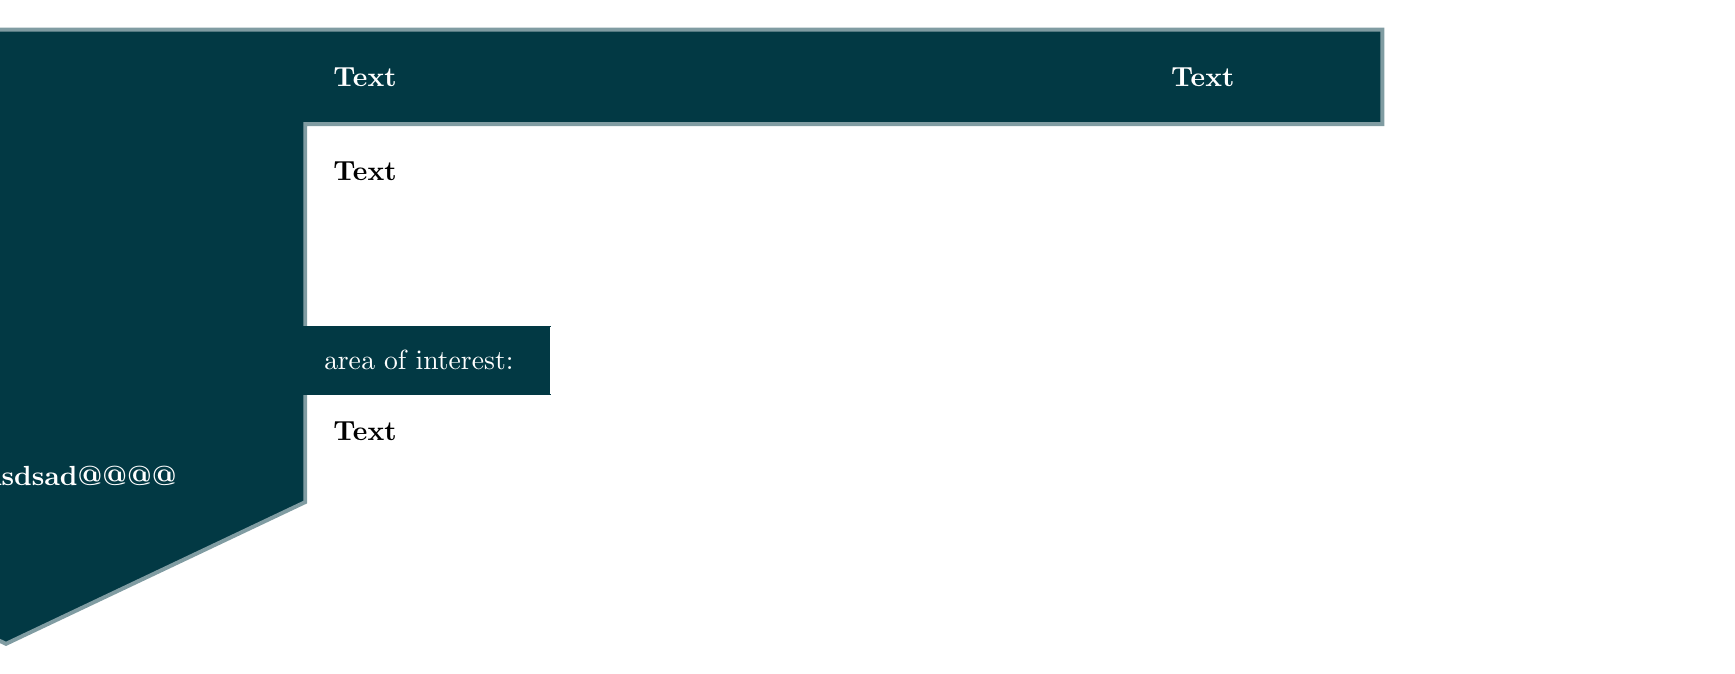
\begin{tikzpicture}[x=1cm ,y=1cm,xscale=0.76, yscale=0.60]
    \voffset = -150pt
    \hspace {-4.1cm}
    \draw (3,0) [line width=0.5mm, Mtrs!50, fill=Mtrs!100] 
    (0,0) -- (0,10) -- (28,10) -- (28,8) -- (10,8)
    -- (10,0) -- (5,-3) -- cycle 
    ; 
    \node at (5,5) {
        \begin{tabular}[t]{p{6cm}}
        \color{white}
        C
        \\
        P
        \\
        ()
        \\
        e-Mail - 
        \\
        git - 
        \\
    \end{tabular} 
    }; 
    \hspace {1cm}
    \draw  (0,0) [line width=0.2mm, MidnightBlue!80, fill=blue!10,
    xscale=0.07, yscale=0.07]
    (6,3) -- (4,1) -- (5,5) -- (7,1) -- (9,2) -- (15,13) -- (5,5) -- (4,1) -- (4,6) -- (15,13) -- (2,9) -- (0,7) -- (4,6) -- cycle ; 
    \node at (3.35,0.5) {\color{white} \bf \href {https://t.me/asdsad}{@@@@}};
 

    \hspace {-1cm}
    \node at (11,9) {\color{white} \bf Text};
    \node at (25,9) {\color{white} \bf Text};
    \node at (11,7) {\color{black} \bf Text}; 

    \setlength{\fboxsep}{0.3cm}
    \node at (120mm,3) {\fcolorbox{Mtrs!100}{Mtrs}{\color{white}
    area of interest: }} ; 

    \node at (11,1.5) {\color{black} \bf Text}; 
    \end{tikzpicture}


\begin{tikzpicture}   
    \hspace {-3em} 
    \draw (0,1) node [copy shadow={draw=gray,fill=Mtrs1!100,opacity=0.4,
                    shadow xshift=0.25ex, shadow yshift=-0.7ex},fill=Mtrs!100,
                    draw=black!15,line width=0.75mm, minimum width=445, 
                    minimum height=7.5mm ] at (0,0)
            {\color{white} \bf EXPERIENCES};
\end{tikzpicture}

\hspace {-3em}
\setlength{ \arrayrulewidth }{ 0,05mm }
\begin{tabular}[t]{p{3em}:p{31em}}
    \hdashline[1pt/1pt]
    2018 – 2019
    & 
    LLC
    \\
    \hdashline[1pt/1pt]
    2018 – 2019 &
    LLC \\
    \hdashline[1pt/1pt]
\end{tabular}


\begin{tikzpicture}   
    \hspace {-3em} 
    \draw (0,0) node [copy shadow={draw=gray,fill=Mtrs1!100,opacity=0.4,
                    shadow xshift=0.25ex, shadow yshift=-0.7ex},fill=Mtrs!100,
                    draw=black!15,line width=0.75mm, minimum width=445, 
                    minimum height=7.5mm ] at (0,0)
            {\color{white} \bf EDUCATION};
\end{tikzpicture}

\hspace {-3em}
\setlength{ \arrayrulewidth }{ 0,05mm }
\begin{tabular}[t]{p{35em}}
    \hdashline[1pt/1pt]
    LLC
    \\
    \hdashline[1pt/1pt]
\end{tabular}


\begin{tikzpicture}   
    \hspace {-3em} 
    \draw (0,0) node [copy shadow={draw=gray,fill=Mtrs1!100,opacity=0.4,
                    shadow xshift=0.25ex, shadow yshift=-0.7ex},fill=Mtrs!100,
                    draw=black!15,line width=0.75mm, minimum width=445, 
                    minimum height=7.5mm ] at (0,0)
            {\color{white} \bf COMPETENCE};
\end{tikzpicture}

\hspace {-3em}
\setlength{ \arrayrulewidth }{ 0,05mm }
\begin{tabular}[t]{p{35em}}
    \hdashline[1pt/1pt]
    Development skills with:
    -
    \\
    -
    \\
    -
    \\
    Profile Github: \href {https://github.com/}{git}
    \\
    \hdashline[1pt/1pt]
\end{tabular}


\begin{tikzpicture}   
    \hspace {-3em} 
    \draw (0,0) node [copy shadow={draw=gray,fill=Mtrs1!100,opacity=0.4,
                    shadow xshift=0.25ex, shadow yshift=-0.7ex},fill=Mtrs!100,
                    draw=black!15,line width=0.75mm, minimum width=445, 
                    minimum height=7.5mm ] at (0,0)
            {\color{white} \bf International languages};
\end{tikzpicture}

\hspace {-3em}
\setlength{ \arrayrulewidth }{ 0,05mm }
\begin{tabular}[t]{p{35em}}
    \hdashline[1pt/1pt]
    LLC
    \\
    \hdashline[1pt/1pt]
\end{tabular}

\end{document}

